\section{Introduction}

\paragraph{Background}

Today we all know that personal computers do not rule the chip industry's market
anymore but it does much more by small intelligent devices. If we look into the
near future upcoming technologies like the internet of things, intelligent cars
or drones will overrule all previous market demands for chip industries. Common
properties of such devices made chip producers already shifting their challenges
from transistor level to core level for following reasons:

\begin{enumerate}
\item Integration of multiple powerful functionalities into one small device
\item Energy efficiency, because of power dissipation in nanoscale VLSI circuits. 
\item Cost reduction due the growth of chip producing competitors in these markets.
\item Time to market improvement by combining intellectual properties into one product.
\end{enumerate}

This background illustrates the importance of further integration and the
related technologies that makes this possible. These technologies are introduced
in the next sections. \cite{SoC-market}

\paragraph{SoC}

An integrated circuit that covers multiple cores or intellectual properties
blocks (IP's) which are linked to an internal bus system is called a system on
chip or SoC. IP's of several companies are integrated into a single chip, by
this a company can focus on its core business instead of building all the
functionality by themselves and reduce time to market. Following Moore's law the
number of IP's in a SoC will double every two years. But the more IP's attached
to a traditional bus system the wiring delay increases exponential and longer
wiring reduces the bus its bandwidth.\cite{SoC}

\paragraph{NoC}

To cope with the increasing number of cores into one chip and to make
integration of IP's from different companies less complex the use of network
communication inside a chip instead of a traditional bus system is inevitable. A
so called network on chip or NoC has much less wiring and can handle more IP's
without losing performance. For the related business it has the same advantage
as it does for network communication in general:

\textit{``Replacement of SoC busses by NoCs will follow the same path of data
communications when the economics prove that the NoC either reduces SoC
manufacturing cost, SoC time to market, SoC time to volume, and SoC design risk
or increases SoC performance.''} \cite{NoC-busses} 

The success of the NoC design depends on the research of the interfaces between
processing elements of NoC and interconnection fabric the performance of the NoC
design relies greatly on the interconnection paradigm.

\paragraph{xMAS}

If a SoC does not meet its specification or isn't reliable e.g. because of
deadlock situations in a NoC, the cost of production loss is much higher than
the costs spent for design or verification. In worst case a company can lose its
market share and remain reputational damage. It is very important to detect
flaws in an early stage of SoC production process, therefor researchers have
developed a high level modelling language for communication fabrics called xMAS
or executable Micro Architectural Specifications. This high level approach makes
it less complex and gives researchers a way to gain knowledge of how these
fabrics behave under certain conditions so they can prove the absence or
presence of specific properties long before it's built on silicon.

xMAS consist of only eight primitive components that have one or more ports. To
create a valid model all ports must be connected by channels and components must
be parameterized. Once a model has been created and parameterized it can be
verified to detect deadlock situations or other flaws. 

\begin{figure}[here]
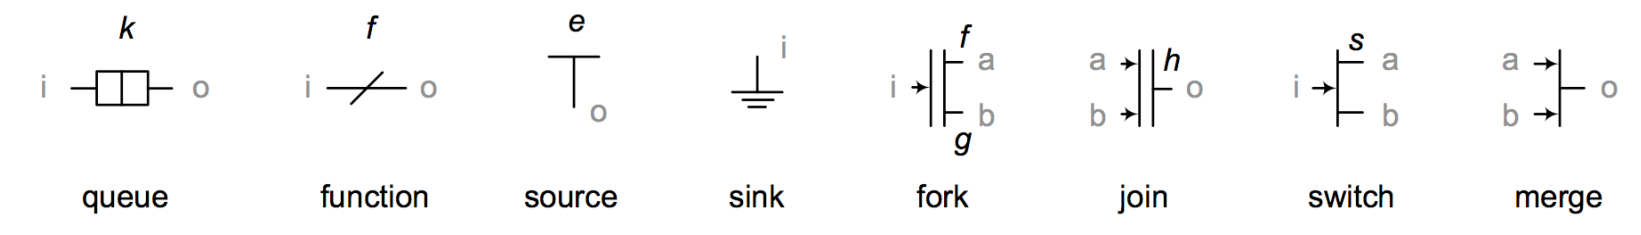
\includegraphics[width=1.0\textwidth]{xmas-language}
\caption{Eight primitives of the xMAS language \cite{6225465}. Italicized letters indicate
parameters. Gray letters indicate ports.}
\label{fig:xmas-language}
\end{figure}

\paragraph{Design and verification tools}

To make use of the xMAS language and verification tools, computer scientists
have developed an application called WickedXMAS \cite{WickedXmas}.
With this application it is possible to draw a model and export it so it can be
verified. The verification tool reads the model and process one or more
algorithms e.g. to detect network deadlocks or model syntax faults.

To stay ahead and because of the importance of pre-production verification, our
team has created a complete new tool. Our goal was to create a maintainable,
platform independent, xMAS modelling tool that integrates the verification
tools. The project is split into a designer that we call ``xmd'' or xMAS Model
Designer and the verification process called ``xmv'' or xMAS Model Verification. The
project is based on Qt's latest technology where we have written the GUI in QML
(JavaScript) and the logic in c++.

Instead of implementing specific verification tools we have put our effort into
implementing a generic plugin interface. Via this interface, verification tools
can be easily plugged in, controlled and send feedback to the designer. 
\begin{wrapfigure}{r}{0.55\textwidth}
  \vspace{-20pt}
  \begin{center}
    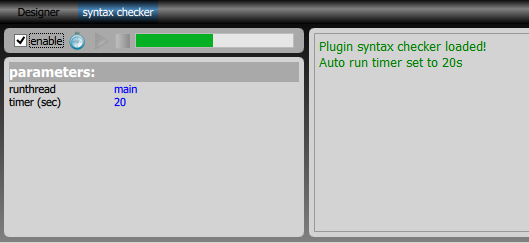
\includegraphics[width=0.50\textwidth]{console}
  \end{center}
  \vspace{-20pt}
  \caption{xmd syntax checker plugin console}
  \label{fig:console}
  \vspace{-10pt}
\end{wrapfigure}
A scientist can easily implement a new verification algorithm if it has the plugin
interface. We've foreseen the syntax checker of such a plugin interface and can
be used as an example. 
Each plugin gets automatically its own console output and
control with setup fields. Starting a verification process is simply done by
clicking the start button, no conversion or exports are necessary anymore.


In the new designer ``xmd'' all actions on the canvas are now directly reflected
into the model network and can be verified immediately. Another improvement of
the designer is the management of composite components, which are subnetworks
that can be reused and make it possible to quickly build large models in an easy
way.
\begin{wrapfigure}{r}{0.55\textwidth}
  \vspace{-20pt}
  \begin{center}
    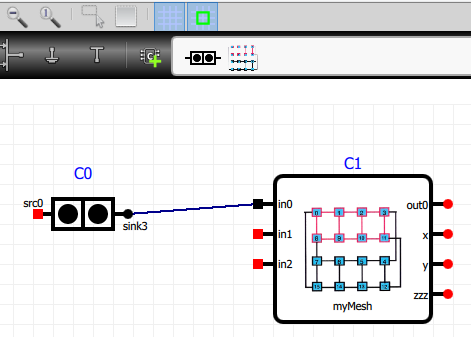
\includegraphics[width=0.50\textwidth]{composite-use}
  \end{center}
  \vspace{-20pt}
  \caption{xmd composite library and canvas use}
\label{fig:composite-use}
  \vspace{-10pt}
\end{wrapfigure}
Models can be setup with composite properties so these can be used just
like primitives. A designer can do this by adding them to a model its composite
library and drag those into the canvas. The way that xmd implements composites
gives scientists the opportunity to extend these with a parametric expression.
With a parametric expression it is possible to call a composite in a recursive
way and avoid drawing large networks of already valid subnets.

\newpage